\documentclass[9pt,twocolumn,twoside]{styles/osajnl}
\usepackage{fancyvrb}
\journal{i524} 

\title{Apache Airavata}

\author[1,*]{Scott McClary}

\affil[1]{School of Informatics and Computing, Bloomington, IN 47408, U.S.A.}

\affil[*]{Corresponding authors: scmcclar@indiana.edu}

\dates{paper-001, \today}

\ociscodes{Cloud, Gateway, HPC, I524, Middlware, Workflow}
\doi{\url{https://github.com/scottmcclary1/sp17-i524/blob/master/paper1/S17-IO-3011/report.pdf}}

\begin{abstract}
Apache Airavata provides an alternative to running and monitoring
large-scale scientific applications from the command line. The Apache
Software Foundation's Airavata software framework allows developers to
create what are known as Science Gateways. These Graphical User
Interfaces are desktop-based and/or web-based applications, which
allow researchers to compose, manage, execute and monitor their
research workflows in a user-friendly manner. Apache Airavata
simplifies the process of accessing the large-scale computational
power of local clusters, supercomputers, computational grids and
computing clouds.
\newline
\end{abstract}

\setboolean{displaycopyright}{true}

\begin{document}

\maketitle

\section{Introduction} \label{introduction}
Apache Airavata is an open-source software framework designed to
diminish the learning curve and reduce the inherent complexity of
conducting large-scale scientific computing. Therefore, scientific
researchers leverage the Apache Airavata software framework in order
to obscure the intricacies of running large-scale applications or
workflows on local clusters, powerful supercomputers or distributed
clouds. The expertise and interests of a given researcher likely
revolves around their specific area of research (i.e. Computational
Chemistry, Molecular Dynamics and etc.). The Apache Airavata
technology allows these researchers to focus their time, effort and
grant money on the science rather than the details of the
computing. In addition to executing and monitoring large-scale
scientific applications, managing the input and visualizing the output
from the command line can be complicated on distributed compute
resources. Apache Airavata provides the technological infrastructure
to make these complicated tasks simple. The general idea is to wrap
command line-driven applications (i.e. Gaussian, Amber, NAMD and etc.)
with Apache Airavata in order to create simple, effective and
efficient Science Gateways. The Apache Airavata software framework
provides the infrastructure to allow Science Gateway developers to
abstract away the described complexity so that end-users can simply
``compose, manage, execute, and monitor large-scale applications and
workflows'' with the click of a button \cite{www-airavata}.

\section{Architecture} \label{architecture}
\begin{figure}[htbp]
\centering
\fbox{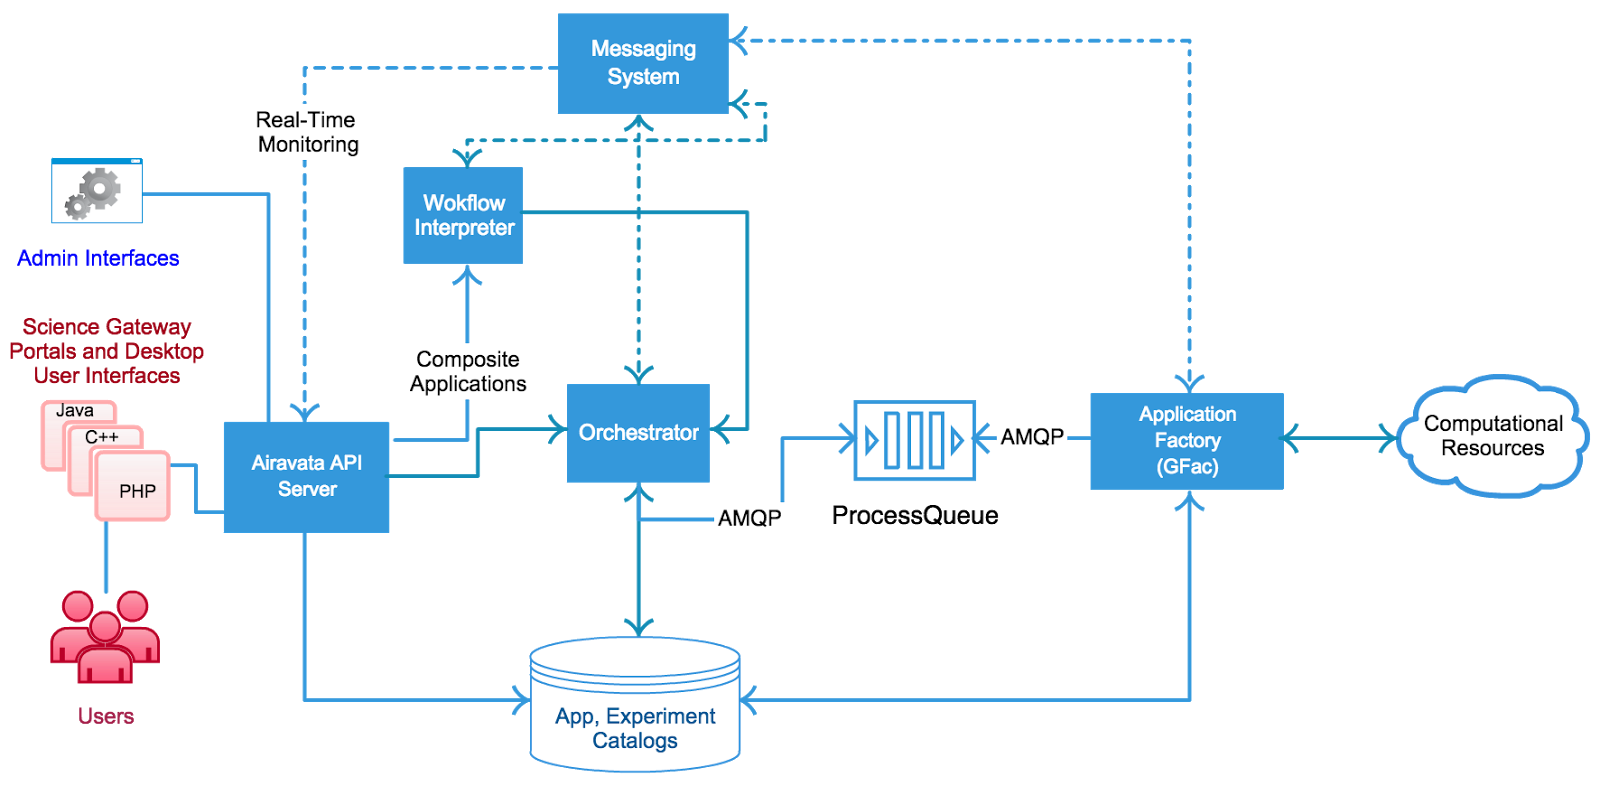
\includegraphics[width=\linewidth]{images/airavata-architecture}}
\caption{The image above depicts the architectural details of Apache
  Airavata \cite{www-documentation}.}
\label{fig:airavata-architecture}
\end{figure}
Figure \ref{fig:airavata-architecture} depicts the architectural
details of Apache Airavata. From this diagram one can see how
end-users are able to interact with the Apache Airavata services (API
Server, Workflow Interpreter, Orchestrator, Messaging System and etc.)
via Science Gateways. The Apache Software foundation provides a
detailed description of the architectural diagram shown in figure
\ref{fig:airavata-architecture} \cite{www-documentation}.

\subsection{API} \label{api}
As introduced in section \ref{ecosystem} and shown with multiple
real-world examples in section \ref{use}, researchers leverage Science
Gateways to interact with Apache Airavata. In order to promote
simplicity, Apache Airavata's application programming interface (API)
is intentionally obscured from these end-users. Therefore, the
Airavata API is generally intended for Science Gateway developers who
are specifically interested in using Apache Airavata as a middleware
service between a user interface and one or more compute resources, as
shown in figure \ref{fig:airavata-ecosystem}. Airavata API is written
using apache thrift \cite{www-documentation}. This allows Science
Gateway developers to use the programming language of their choice
(e.g. Java, PHP, JavaScript, C++, etc.). The Apache Software Foundation
provides an in-depth overview of the API for those interested in
learning the details of this service \cite{www-api}.

\subsection{Shell Access} \label{shell}
As section \ref{introduction} thoroughly explained, Apache Airavata's
purpose is to simplify the typical command line driven process of
composing, managing, executing, and monitoring large-scale scientific
applications on powerful distributed computing resources. Therefore,
end-users of Apache Airavata should not rely on shell access. Instead,
section \ref{graphical} explains that end-users interact with Apache
Airavata through graphical interfaces (i.e. Science Gateways). Shell
access is contained to the Science Gateway developer level of the
technological ecosystem, shown in figure \ref{fig:airavata-ecosystem}.

\subsection{Graphical Interface} \label{graphical}
Apache Airavata leverages a Graphical Workflow Composer, known as
XBaya, which helps ``create workflows, submit and manage multiple
applications ... [and] also has a web-based interface ... where users
can ... register, run and monitor applications ''
\cite{www-documentation}. Furthermore, the Apache Airavata's
thrift-based API, introduced and discussed in section \ref{api},
allows developers to create their own desktop and web interfaces using
Airavata as the technological foundation.

\subsubsection{Science Gateways} \label{science}
Science Gateways are the resulting reward of leveraging Apache
Airavata. As explained in \ref{ecosystem}, Science Gateways are an
instrumental piece of the Apache Airavata ecosystem that allow end
users to compose, manage, execute, and monitor scientific research
workflows on distributed (and potentially complex) compute
resources. Science Gateways simplify workflows and allow researchers
to focus their expensive time and effort on science. Furthermore,
Science Gateways promote reproducibility, which is an important piece
of scientific research as well as publication. In other words, it is
beneficial to researchers to have the ability to easily reproduce
results from an experiment in the past and Science Gateways typically
ensure this functionality. Section \ref{use} describes many of the
prominent and currently available Science Gateways built on top of the
Apache Airavata software framework.

\section{Licensing} \label{licensing}
Apache Airavata is open source software \cite{www-source}. Therefore,
anyone can download, install, modify and improve this software
framework using the popular ``fork and pull'' model. As part of an
introductory tutorial, one can create an Airavata Test Drive account,
which is free as well. Note, this free Airavata Test Drive account
will need to be approved by an Airavata Test Drive Administrator
before one can use the system. Once this approval occurs, one can
simply create and run ``experiments'' (i.e. Gaussian, Amber, Trinity
and etc.) via a Science Gateway on local clusters, supercomputers,
computational grids and computing clouds.

\section{Ecosystem} \label{ecosystem}
\begin{figure}[htbp]
\centering
\fbox{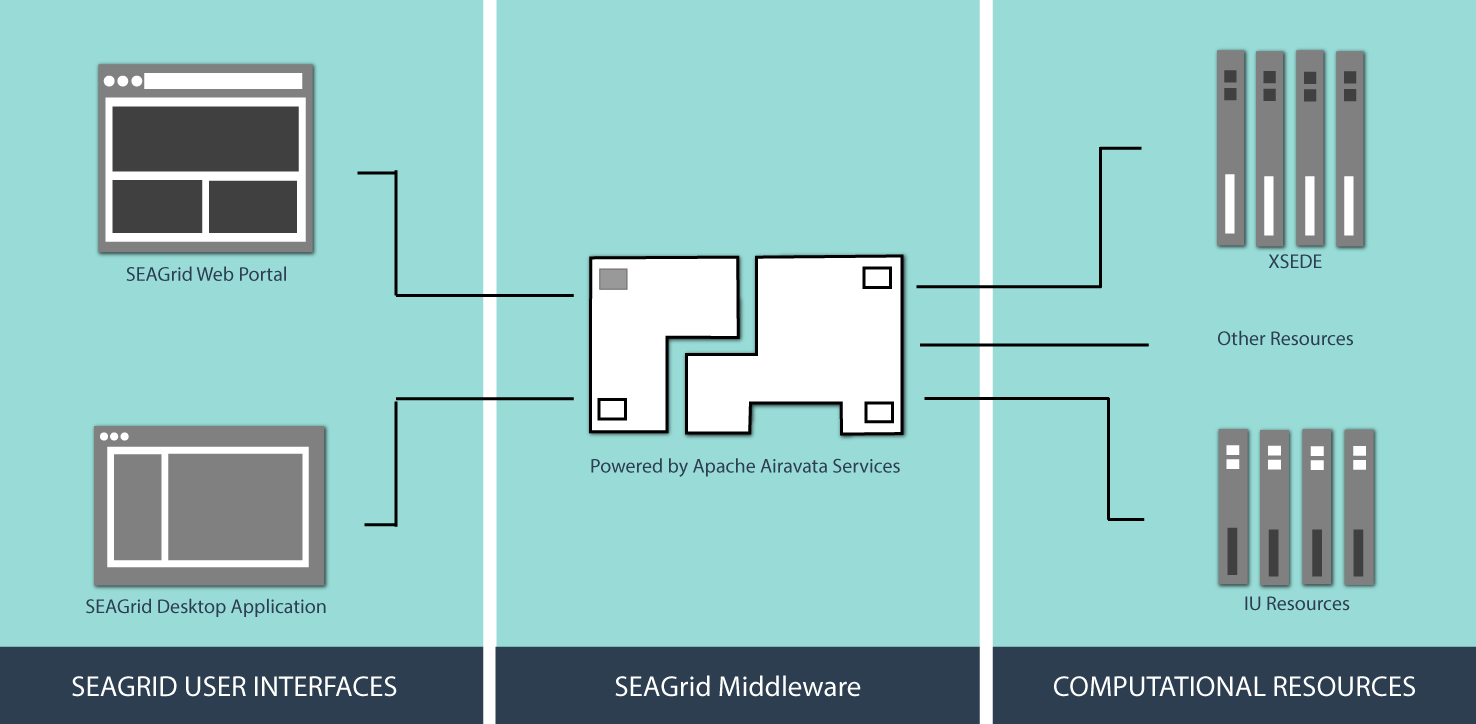
\includegraphics[width=\linewidth]{images/airavata-ecosystem}}
\caption{The image above depicts an example of the technological
  ecosystem developed around Airavata \cite{www-airavata-ecosystem}.}
\label{fig:airavata-ecosystem}
\end{figure}
Figure \ref{fig:airavata-ecosystem} depicts the ecosystem developed
around Apache Airavata for SEAGrid. Apache Airavata plays an important role as the
middleware between the end-users (Science Gateways) and the compute
resources. As discussed above, the placement of Apache Airavata in
between the compute resources and the science gateways allows for the
abstraction of the complexity of composing, running, executing and
managing applications and workflows.

\section{Use Cases} \label{use}
Ultrascan \cite{www-ultrascan}, SEAGrid \cite{www-seagrid} and GenApp
\cite{www-genapp} are instances of Science Gateways that leverage
Apache Airavata to perform computations \cite{www-airavata}. Each of
these services is in place to simply bridge the gap between
scientific applications on large-scale compute resources and domain
specialists. In other words, these Science Gateways are examples of
Apache Airavata enabling science.

\subsection{SEAGrid} \label{seagrid}
The Apache Airavata services allow Science Gateways such as SEAGrid to
simplify the use of ``scientific applications deployed across a wide
range of supercomputers, campus clusters and computing cloud''
\cite{www-seagrid}. SEAGrids bridges the gap between domain
specialists and scientific applications on large-scale compute
resources using both a desktop client and web application. SEAGrid
currently promotes research in Computational Chemistry (e.g. Gaussian,
Gamess, etc.), Molecular Dynamics (Lammps, Amber, NAMD and etc.),
Structural Mechanics (e.g. Abaqus and etc.), Fluid Dynamics
(e.g. Nek5000, OpenFOAM and etc.) and much more. SEAGrid abstracts
away the fine-grained details of running such scientific applications
on large-scale compute resources and therefore allows the domain
specialists to focus on the fine-grained details of their scientific
research. Additionally, SEAGrid enables scientists to create model
inputs, visualizations of outputs and archives for simulation data''
\cite{www-seagrid}.

\subsection{Use Cases for Big Data} \label{big}
The One-Degree Imager (ODI) ``is a gigapixel mosaic camera ... built
by [the] WIYN Observatory with a pixel scale of 0.1 arcseconds for the
3.5-meter telescope'' and is the newest instrument at the WIYN 3.5m
Observatory in Sells, AZ \cite{www-odi, www-wiyn}. Similarly to the
SEAGrid Science Gateway, the Apache Airavata software framework is at
the foundation of ODI's Pipeline, Portal and Archive (PPA) system
which ``execute[s] the NOAO High Performance Pipeline System (NHPPS)
pipelines on XSEDE resources'' \cite{www-odi}. The large amount of
data generated by the ODI demonstrates that the ODI-PPA Science
Gateway and therefore the Apache Airavata software framework can
handle big data software projects. 

\section{Educational material} \label{educational}
There are multiple ways to find out more information about the Apache
Airavata software framework \cite{www-airavata}. In order to cater to
varying audiences and learning styles there is online documentation
\cite{www-documentation}, a course provided at Indiana University,
Bloomington \cite{www-class} as well as online tutorials
\cite{www-tutorial}. The online documentation is entirely sufficient
for motivated users to teach themselves. The online tutorials provide
everything from quick-start to extended tutorials and everything in
between. Historically, there has been a basic Airavata course at
Indiana University offered during the Fall semester and a more
advanced version of the course is offered during the Spring semester.

\section{Conclusion} \label{conclusion}
Apache Airavata appeals to a wide range of scientific researchers
since the technology allows researchers to focus their time, effort
and grant money on the science rather than the details of the
computing. Apache Airavata has enabled researchers to compose, manage,
execute and monitor workflows on large-scale systems with the click of
a button. Gateways such as Ultrascan, SEAGrid and GenApp are clear and
defined examples of how Apache Airavata has been leveraged to improve
and optimize scientific research workflows. As compute resources get
more complicated and/or distributed over time, the Apache Airavata
software framework will continue to promote the ease of use with
Science Gateways.

\section*{Acknowledgements}
The authors would like to thank the School of Informatics and
Computing for providing the Big Data Software and Projects (INFO-I524)
course \cite{www-i524}. This paper would not have been possible
without the technical support \& edification from Gregor von Laszewski
and his distinguished colleagues.

 
\section*{Author Biographies}
\begingroup
\setlength\intextsep{0pt}
\begin{minipage}[t][3.2cm][t]{1.0\columnwidth} 
  \begin{wrapfigure}{L}{0.25\columnwidth}
    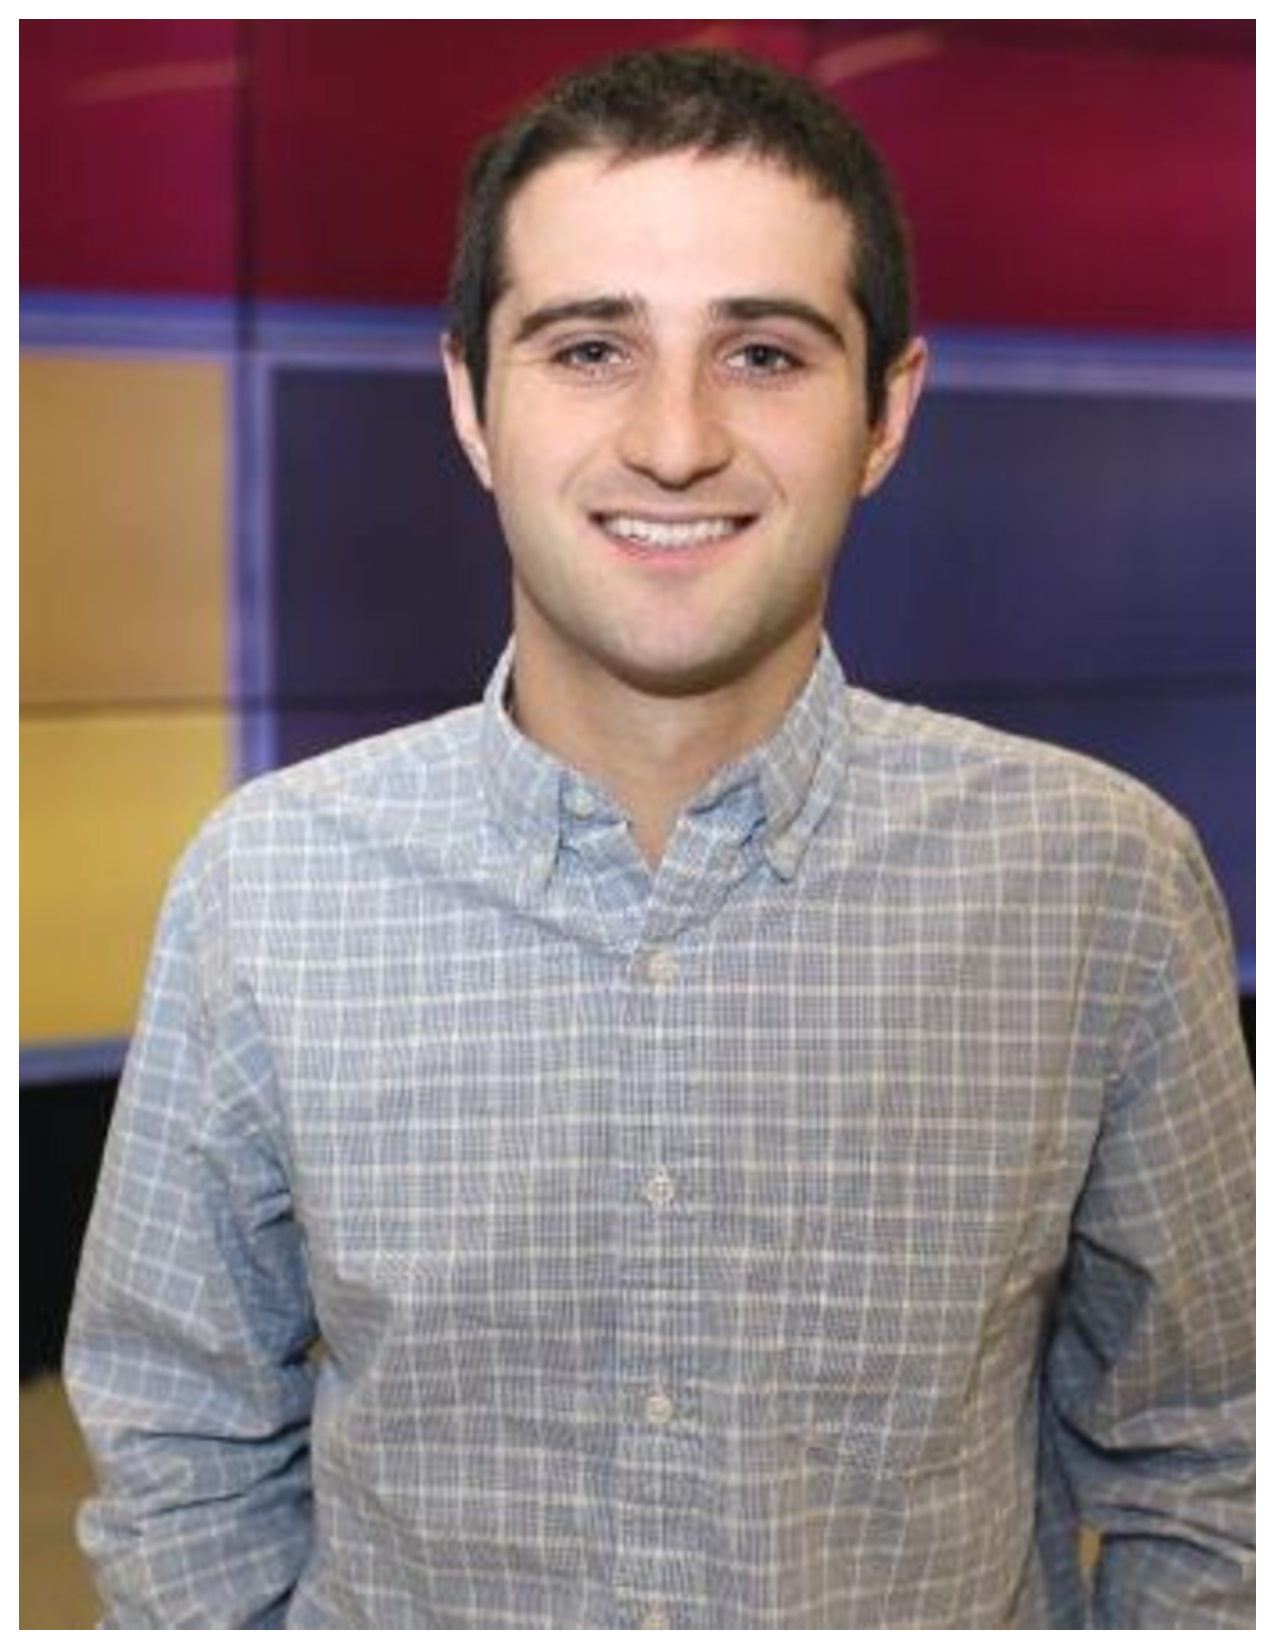
\includegraphics[width=0.25\columnwidth]{images/scott_mcclary}
  \end{wrapfigure}
  \noindent
  {\bfseries Scott McClary} received his BSc (Computer Science) and
  Minor (Mathematics) in May 2016 from Indiana University and will
  receive his MSc (Computer Science) in May 2017 from Indiana
  University. His research interests are within scientific application
  performance analysis on large-scale HPC systems. He will begin
  working as a Software Engineer with General Electric Digital in San
  Ramon, CA in July 2017.
\end{minipage}
\endgroup

\section*{} %used to create more spacing..
\section*{Work Breakdown}
The work on this project was distributed as follows between the
authors:
\begin{description}
\item[Scott McClary.] He completed all of the work for this paper
  including researching and testing Apache Airavata as well as
  composing this technology paper.
\end{description}

% Bibliography
\bibliography{references}
\end{document}

